% Source printed pp. 242-253 / PDF pp. 250-261.
\section{\texorpdfstring{稳定约化与 $\overline{\mathcal M}_{g,\allowbreak n}$ 的固有性}{稳定约化与 稳定曲线模叠 的固有性}}\label{src:6.5}
\begin{epigraph}
代数曲线是上帝创造的, 而代数曲面是魔鬼创造的.
\epigraphauthor{Max Noether}
\end{epigraph}
我们讨论 Deligne 和 Mumford 关于 $\overline{\mathcal M}_{g,\allowbreak n}$ 固有性的著名定理~\cite{DM69}. 关键是稳定约化定理.
\begin{theorem}[稳定约化]\label{src:6.5.1}
设 $R$ 是离散赋值环, $K=\operatorname{Frac}(R)$, 并置 $\Delta=\Spec R$, $\Delta^*=\Spec K$. 若 $(\mathcal C^*\to\Delta^*,\allowbreak \sigma_1^*,\allowbreak \ldots,\allowbreak \sigma_n^*)$ 是 $n$-点稳定曲线族, 则存在离散赋值环的扩张 $R\to\allowbreak R'$ 及 $n$-点稳定曲线族 $(\mathcal C\to\Delta'=\Spec R',\allowbreak \sigma_1,\allowbreak \ldots,\allowbreak \sigma_n)$, 延拓 $(\mathcal C^*\to\Delta^*,\allowbreak \sigma_1^*,\allowbreak \ldots,\allowbreak \sigma_n^*)$ 到 $K'=\operatorname{Frac}R'$ 的基变换.
\end{theorem}
定理对任意离散赋值环成立, 但本节仅在特征 $0$ 下给出完整证明, 遵循~\cite[第 II 章]{KKMS73}, \cite[\S3.C]{HM98} 和~\cite[\S X.4]{ACG11}.
\begin{remark}\label{src:6.5.2}
特征 $0$ 下的稳定约化定理最早陈述于~\cite[引理 A]{MM64b}, 证明概要见~\cite{May69}. 一般版本首次出现于 Deligne 和 Mumford 的开创性论文~\cite{DM69}. 他们将一般纤维 $C^*$ 嵌入其 Jacobian, 利用~\cite{SGA7-I,SGA7-II} 中已建立的阿贝尔簇的半稳定约化. Gieseker 用 GIT 给出了另一证明~\cite{Gie82}; 正如~\cite[Tag 0C2Q]{SP} 所说, ``这是一项相当惊人的成就: 不真正研究正维基底上的曲线族就能证明这样的结果, 似乎有些违反直觉.'' 后来 Artin--Winters~\cite{AW71} 和 Saito~\cite{Sai87} 的论证大体遵循这里的策略, 但在正特征下需要更多技术; 见注记~\bookref{6.5.10}.
\end{remark}
\subsection{稳定约化的证明}\label{src:6.5.1-subsection}
以下始终令 $\Delta=\Spec R$, 其中 $R$ 是定义在 $\mathbb Q$ 上的离散赋值环; 令 $\Delta^*=\Spec K$, 其中 $K=\operatorname{Frac}(R)$; 令 $t\in R$ 为一致化参数, $0=(t)\in\Spec R$ 为唯一闭点. 给定亏格为 $g$ 的 $n$-点稳定曲线族 $(\mathcal C^*\to\Delta^*,\allowbreak \sigma_1^*,\allowbreak \ldots,\allowbreak \sigma_n^*)$.

\noindent\textbf{证明策略}
\begin{enumerate}[(1)]
\item 归结到 $\mathcal C^*\to\Delta^*$ 光滑的情形.
\item 构造平坦延拓 $\mathcal C\to\Delta$.
\item 将 $\mathcal C$ 换为奇点消解, 使约化中心纤维 $(\mathcal C_0)_{\mathrm{red}}$ 仅有结点.
\item 作分歧基扩张 $\Delta'\to\Delta$, 使 $\mathcal C\times_\Delta\Delta'$ 的正规化具有约化中心纤维.
\item 使标记点光滑且互异.
\item 收缩中心纤维中的有理尾和有理桥.
\end{enumerate}
阅读证明时记住一些例子会很有帮助. 一个极简单的例子是 $\mathbb P^2\times\Delta^*$ 中由方程
\begin{equation}\label{src:6.5.3}
y^2z=x(x-z)(x-tz)
\end{equation}
及截面 $\sigma^*(t)=[0,\allowbreak 1,\allowbreak 0]$ 定义的椭圆曲线族 $(\mathcal C^*\to\Delta^*,\allowbreak \sigma^*)$. 此时, 从 $\mathcal C^*$ 的描述便可看出稳定极限: 由~\bookeqref{6.5.3} 定义 $\mathcal C\subseteq\mathbb P^2\times\Delta$, 并取 $\sigma(t)=[0,\allowbreak 1,\allowbreak 0]$, 则 $(\mathcal C\to\Delta,\allowbreak \sigma)$ 是延拓 $(\mathcal C^*\to\Delta^*,\allowbreak \sigma^*)$ 的稳定族; 见图~\bookref{1.7.3}. 稳定极限 $\mathcal C_0$ 是结点三次曲线 $y^2z=x^2(x-z)$. 证明中还给出其他例子, 更复杂的例子见~\bookref{6.5.2-subsection} 节.
\begin{proof}[特征 $0$ 下稳定约化定理 (\bookref{6.5.1}) 的证明]
\textbf{步骤 $1$: 归结到 $\mathcal C^*\to\Delta^*$ 光滑的情形.}
若 $\mathcal C^*$ 有 $\delta$ 个结点, 则将 $K$ 和 $R$ 换为扩张后, 可使第 $j$ 个结点由 $K$-点 $n_j^*\in\mathcal C^*$ 给出, 且它在正规化 $\widetilde{\mathcal C}^*\to\mathcal C^*$ 下的原像由两个 $K$-点 $q_j^*$, $r_j^*$ 组成. 称 $(\widetilde{\mathcal C}^*\to\Delta^*,\allowbreak \sigma_i^*,\allowbreak q_j^*,\allowbreak r_j^*)$ 为带标记的正规化. 令 $(\widetilde{\mathcal C}_k^*\to\Delta^*,\allowbreak q_{kl}^*)$ 为带标记的连通分支, 其中 $\{q_{kl}^*\}=\{\sigma_i^*,\allowbreak q_j^*,\allowbreak r_j^*\}\cap\widetilde{\mathcal C}_k^*$. 由于 $\mathcal C^*$ 稳定, 每个 $(\widetilde{\mathcal C}_k^*\to\Delta^*,\allowbreak q_{kl}^*)$ 也稳定 (习题~\bookref{6.3.7}).

假定一般纤维 $\mathcal C^*$ 光滑时稳定约化成立, 则将 $K$ 和 $R$ 换为扩张后, 可构造延拓 $(\widetilde{\mathcal C}_k^*\to\Delta^*,\allowbreak q_{kl}^*)$ 的稳定族 $(\widetilde{\mathcal C}_k\to\Delta,\allowbreak q_{kl})$. 对每个 $j=1,\allowbreak \ldots,\allowbreak \delta$, 用 Ferrand 推出 (\bookref{B.4.1}) 粘合对应于 $q_j^*$ 和 $r_j^*$ 的截面 $q_{il}$, $q_{i'l'}$. 由光滑态射的平展局部结构 (命题~\bookref{A.3.4}) 和推出的平展局部性质 (命题~\bookref{B.4.8}(3)), 推出具有形如
\[
\begin{tikzcd}[column sep=large]
\Spec R\amalg\Spec R\arrow[r,"0\amalg0"]\arrow[d]&\mathbb A_R^1\amalg\mathbb A_R^1\arrow[d]\\
\Spec R\arrow[r]\arrow[ur,phantom,"\lrcorner"]&\Spec A
\end{tikzcd}
\qquad
\begin{aligned}
A&=R\times_{R\times R}(R[x]\times R[y])\\
 &=\{(f,g)\in R[x]\times R[y]\mid f(0)=g(0)\}\\
 &=R[x,y]/(xy)
\end{aligned}
\]
的平展邻域. 截面 $q_{il}$ 和 $q_{i'l'}$ 被粘成结点, 得到带有 $\delta$ 个选出结点的附加截面的 $n$-点结点曲线族 $(\mathcal C\to\Delta,\allowbreak \sigma_i)$. 中心纤维 $\mathcal C_0$ 的带标记正规化是中心纤维 $(\widetilde{\mathcal C}_k)_0$ 的不交并; 由习题~\bookref{6.3.7}, $(\mathcal C_0,\allowbreak \sigma_i(0))$ 稳定. 因而 $(\mathcal C\to\Delta,\allowbreak \sigma_i)$ 是稳定族.
\begingroup\renewcommand{\thefigure}{6.5.3}\renewcommand{\theHfigure}{6.5.3-figure}
\begin{figure}[H]\centering\begin{tikzpicture}
\node[inner sep=0,anchor=south west] (im) at (0,0) {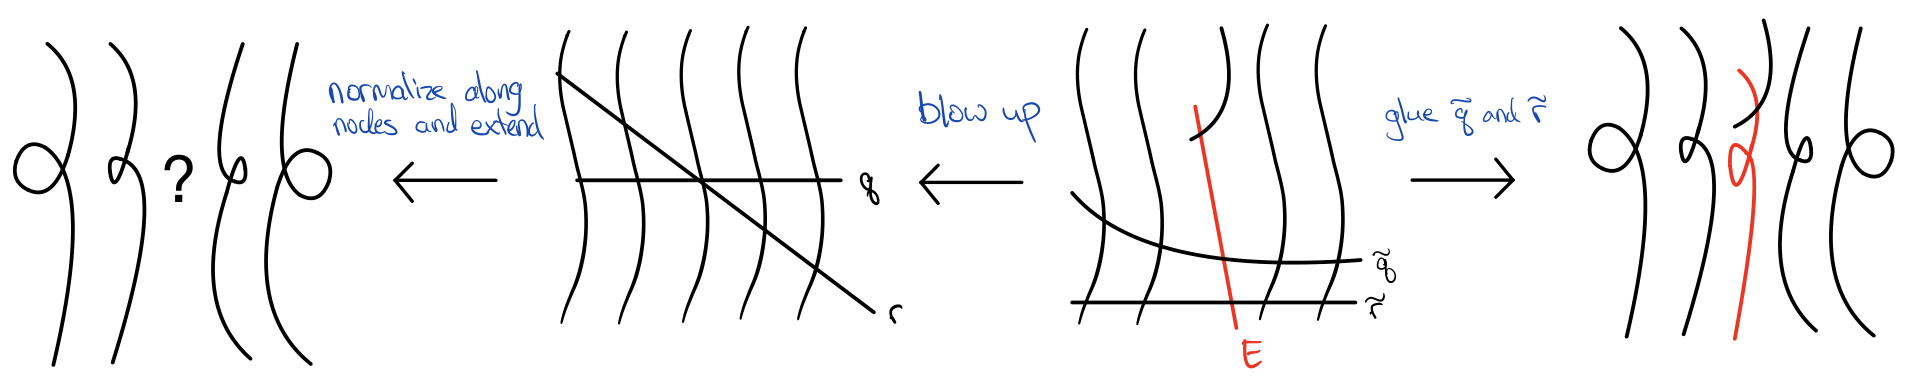
\includegraphics[width=.86\textwidth]{figures/reduction-step1.png}};
\begin{scope}[x={(im.south east)},y={(im.north west)}]
\fill[white] (0.17,0.62) rectangle (0.29,0.84);
\fill[white] (0.47,0.65) rectangle (0.56,0.8);
\fill[white] (0.72,0.64) rectangle (0.83,0.8);
\node[fill=white,inner sep=1pt,font=\scriptsize,text=blue] at (0.23,0.75) {沿结点正规化};
\node[fill=white,inner sep=1pt,font=\scriptsize,text=blue] at (0.23,0.64) {并延拓};
\node[fill=white,inner sep=1pt,font=\scriptsize,text=blue] at (0.514,0.7) {爆破};
\node[fill=white,inner sep=1pt,font=\scriptsize,text=blue] at (0.774,0.7) {粘合 $\widetilde q,\widetilde r$};
\end{scope}\end{tikzpicture}

\caption{(步骤 $1$) 考虑具有一个结点的稳定曲线族 $\mathcal C^*\to\Delta^*$, 例如由 $y^2=x^3+tx^2$ 局部定义的结点退化为尖点. 沿结点正规化, 延拓 $2$-点曲线族, 在截面 $q$, $r$ 的交点处爆破, 再粘合严格变换 $\widetilde q$, $\widetilde r$, 即得稳定极限. 若正规化 $\widetilde{\mathcal C}^*=C\times\Delta^*$ 是常值族, 则稳定极限是 $C$ 与一条有理结点曲线的结点并.}\label{src:6.5.3-figure}
\end{figure}\endgroup\addtocounter{theorem}{-1}
另一种归结方式是利用 $\mathcal M_{g,\allowbreak n}\subseteq\overline{\mathcal M}_{g,\allowbreak n}$ 稠密 (定理~\bookref{6.7.30}): 习题~\bookref{5.6.7} 断言, 只需在 $\Delta^*\to\overline{\mathcal M}_{g,\allowbreak n}$ 经过 $\mathcal M_{g,\allowbreak n}$ 分解的条件下检验固有性的赋值判据.

\textbf{步骤 $2$: 找到平坦延拓 $(\mathcal C\to\Delta,\allowbreak \sigma_i)$.}
由 $(\omega_{\mathcal C^*/\Delta^*}(\sum_i\sigma_i^*))^{\otimes3}$ 甚丰沛 (命题~\bookref{6.3.23}), 可将 $\mathcal C^*$ 嵌入为 $\mathbb P^N\times\Delta^*$ 的闭子概形. 由光滑曲线上的平坦性判据 (\bookref{A.2.2}), $\mathcal C^*\hookrightarrow\mathbb P^N\times\Delta$ 的概形论像 $\mathcal C$ 在 $\Delta$ 上平坦 (因为取闭包不会在中心纤维中引入嵌入点). 这给出延拓 $\mathcal C^*\to\Delta^*$ 的曲线族 $\mathcal C\to\Delta$. (这与命题~\bookref{2.4.2} 中用赋值判据证明 Hilbert 概形固有性的论证相同.) 由固有性的赋值判据 (\bookref{A.4.5}), 截面 $\sigma_i^*: \Delta^*\to\mathcal C^*$ 延拓为截面 $\sigma_i:\Delta\to\mathcal C$.

此时中心纤维 $\mathcal C_0$ 可能具有很严重的奇点, 标记点 $\sigma_i(0)\in\mathcal C_0$ 可能是奇点且彼此重合.
\begin{figure}[H]\centering\begin{tikzpicture}
\node[inner sep=0,anchor=south west] (im) at (0,0) {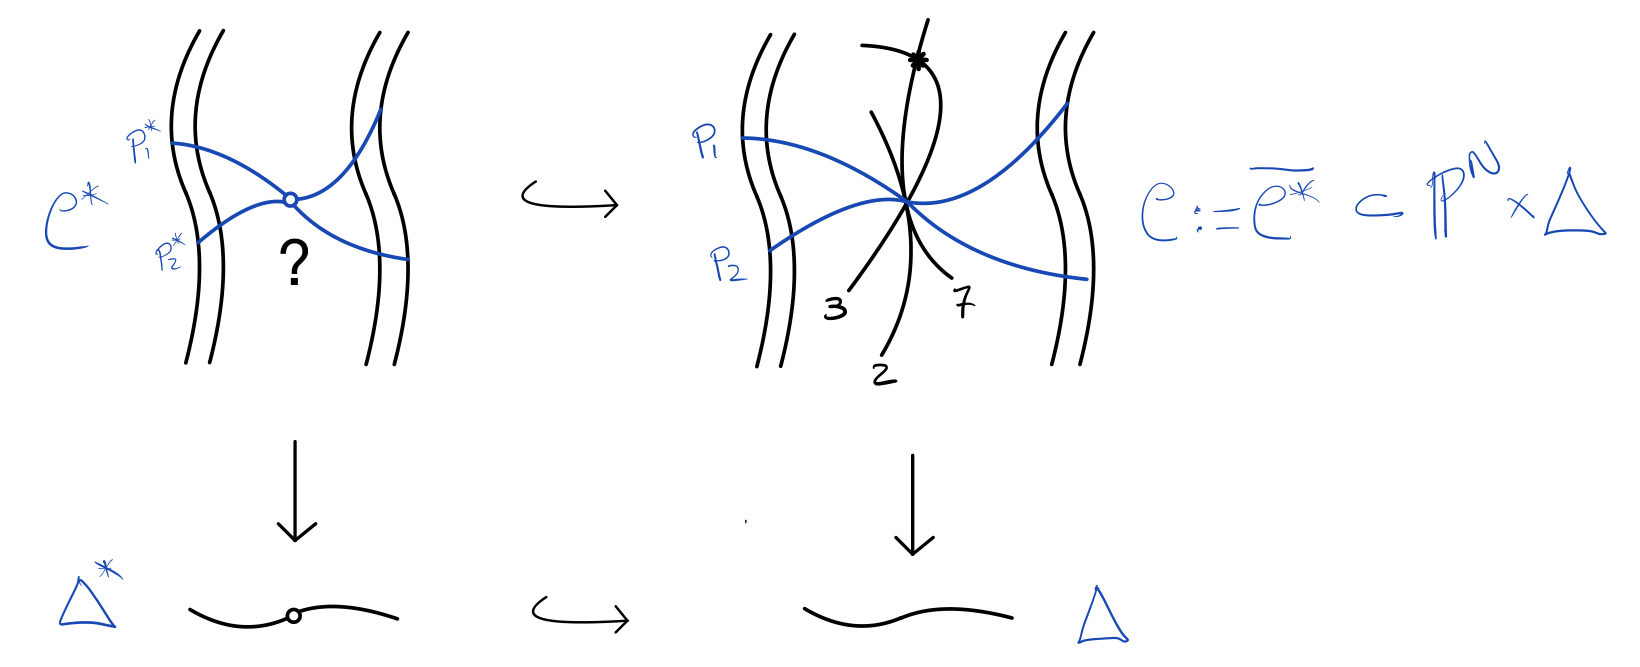
\includegraphics[width=.86\textwidth]{figures/reduction-step2.png}};
\begin{scope}[x={(im.south east)},y={(im.north west)}]


\end{scope}\end{tikzpicture}
\bookfiguretarget{6.5.4}
\caption{(步骤 $2$) 闭包 $\mathcal C:=\overline{\mathcal C^*}$ 是 $\Delta$ 上的平坦族. 中心纤维 $\mathcal C_0$ 可能一般非约化并带有嵌入点; 数字 $3$, $2$, $7$ 表示不可约分支的重数. 标记点 $\sigma_i(0)\in\mathcal C_0$ 可能是奇点且彼此重合.}\bookfigurehref{6.5.4}\label{src:6.5.4}
\end{figure}
\textbf{步骤 $3$: 将 $\mathcal C$ 换为奇点消解, 使约化中心纤维 $(\mathcal C_0)_{\mathrm{red}}$ 仅有结点.}
结合消解的存在性 (\bookref{B.2.1}) 与嵌入消解的存在性 (\bookref{B.2.3}), 存在从正则概形出发的射影双有理态射 $\widetilde{\mathcal C}\to\mathcal C$, 它在 $\Delta^*$ 上是同构, 且中心纤维 $\widetilde{\mathcal C}_0$ 在集合意义下具有正规交叉, 即 $(\widetilde{\mathcal C}_0)_{\mathrm{red}}$ 仅有结点. 由光滑曲线上的平坦性判据 (\bookref{A.2.2}), $\widetilde{\mathcal C}\to\Delta$ 平坦. 将 $\mathcal C$ 换为 $\widetilde{\mathcal C}$, 截面 $\sigma_i$ 换为严格变换.
\begin{figure}[H]\centering\begin{tikzpicture}
\node[inner sep=0,anchor=south west] (im) at (0,0) {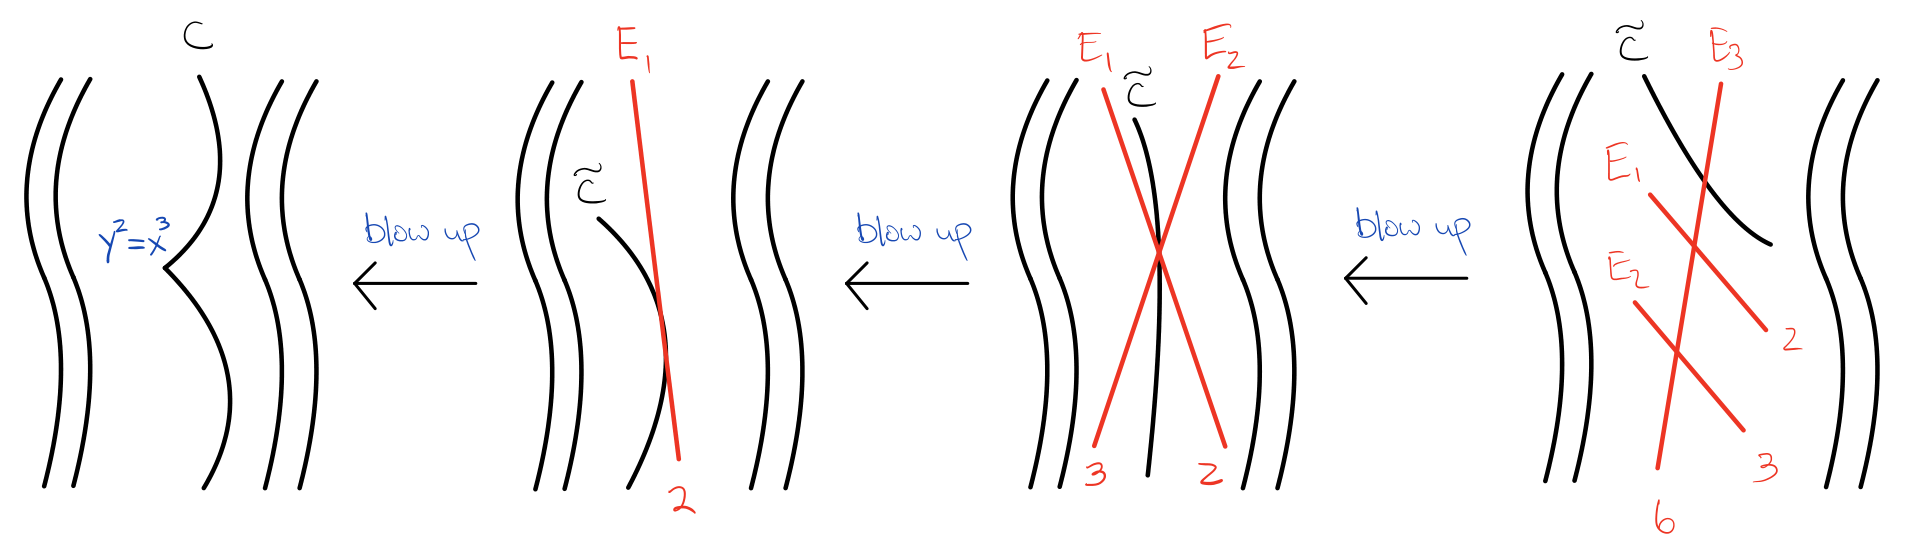
\includegraphics[width=.86\textwidth]{figures/reduction-step3.png}};
\begin{scope}[x={(im.south east)},y={(im.north west)}]
\fill[white] (0.185,0.52) rectangle (0.26,0.65);
\fill[white] (0.44,0.52) rectangle (0.52,0.65);
\fill[white] (0.7,0.52) rectangle (0.78,0.65);
\node[fill=white,inner sep=1pt,font=\scriptsize,text=blue] at (0.21,0.59) {爆破};
\node[fill=white,inner sep=1pt,font=\scriptsize,text=blue] at (0.477,0.59) {爆破};
\node[fill=white,inner sep=1pt,font=\scriptsize,text=blue] at (0.737,0.59) {爆破};
\end{scope}\end{tikzpicture}

\caption{(步骤 $3$) 设 $\mathcal C\to\Delta=\Bbbk[t]_{(t)}$ 是一般光滑的族, 中心纤维退化出尖点 $y^2=x^3$, 且 $\mathcal C$ 在该奇点附近的局部方程为 $y^2=x^3+t$. 反复爆破中心纤维的奇点, 在原曲面上取局部坐标 $x,\allowbreak y$, 在新曲面上取 $\widetilde x,\allowbreak \widetilde y$. 爆破的第一个坐标片中 $\widetilde x=x$, $\widetilde y=y/x$, 例外除子为 $\widetilde x=0$; 第二个坐标片中 $\widetilde x=x/y$, $\widetilde y=y$, 例外除子为 $\widetilde y=0$.}\label{src:6.5.5}
\end{figure}
\begin{itemize}
\item 第一次爆破中, 奇点在第一个坐标片中的原像由 $\widetilde x^2(\widetilde y^2-\widetilde x)$ 给出, 在第二个坐标片中由 $\widetilde y^2(1-\widetilde x^3\widetilde y)$ 给出. 例外除子 $E_1$ 的重数为 $2$. $C$ 的正规化 $\widetilde C$ 的亏格为 $g-1$.
\item 第二次爆破的坐标片由 $\widetilde x^3(\widetilde x\widetilde y^3-1)$ 和 $\widetilde x^2\widetilde y^3(\widetilde y-\widetilde x)$ 定义, 新例外除子 $E_2$ 的重数为 $3$.
\item 最后一次爆破的坐标片为 $\widetilde x^6\widetilde y^3(\widetilde y-1)$ 和 $\widetilde x^2\widetilde y^6(1-\widetilde x)$, 新例外除子 $E_3$ 的重数为 $6$. 中心纤维非约化, 其约化仅有结点.
\end{itemize}
\textbf{步骤 $4$: 作分歧基扩张 $\Delta'=\Spec R'\to\Spec R=\Delta$, 使 $\mathcal C\times_\Delta\Delta'$ 的正规化的中心纤维约化且仅有结点.}
这是最困难的步骤, 特征 $0$ 的假设用在这里. 此论证可看作 Abhyankar 温和分歧引理的一个版本 (见~\cite[\S XIII.5]{SGA1} 和~\cite[Tag 0EXT]{SP}). 因为 $\mathcal C$ 正则, $t\in R$ 不是零因子, 中心纤维 $\mathcal C_0$ 是 Cohen--Macaulay 的, 因而无嵌入点. 另一方面, $(\mathcal C_0)_{\mathrm{red}}$ 是有效 Cartier 除子, 局部由单个方程切出. 对每个 $p\in\mathcal C_0$, 可取平展邻域及局部坐标 $x,\allowbreak y$, 使 $\mathcal C\to\Delta$ 明确描述如下:
\begin{itemize}
\item 若 $p\in(\mathcal C_0)_{\mathrm{red}}$ 是光滑点, 则 $(x,\allowbreak y)\mapsto x^a$, 包含 $p$ 的不可约分支的重数为 $a$;
\item 若 $p\in(\mathcal C_0)_{\mathrm{red}}$ 是结点, 则 $(x,\allowbreak y)\mapsto x^ay^b$, 包含 $p$ 的两个分支的重数为 $a$, $b$. 若 $p$ 是非分离结点 (即 $\mathcal C_0\setminus p$ 连通), 则 $a=b$.
\end{itemize}
令 $N$ 为 $\mathcal C_0$ 的不可约分支重数的最小公倍数. 将 $R$ 换为扩张后, 可假设 $R$ 含有本原 $N$ 次单位根 $\rho$. 令 $\Delta'=\Spec R'\to\Spec R=\Delta$ 为 $N$ 次全分歧离散赋值环扩张 (即一致化参数 $t\in R$ 的像为 $t'^N$, 其中 $t'\in R'$ 是一致化参数). 令 $\mathcal C'=\mathcal C\times_\Delta\Delta'$, $p'\in\mathcal C'$ 为 $p$ 的唯一原像, $\widetilde{\mathcal C}'$ 为 $\mathcal C'$ 的正规化.

若 $p\in(\mathcal C_0)_{\mathrm{red}}$ 光滑, 则 $\mathcal C'$ 在 $p'$ 附近平展局部由 $x^a=t^N$ 定义. 因为 $R$ 的特征为 $0$, 有互异因子分解
\[
x^a-t^N=\prod_{i=0}^{a-1}\bigl(x-(\rho^it)^{N/a}\bigr).
\]
(若特征为正且整除 $N$, 则 $\mathcal C'$ 非约化.) 在正规化 $\widetilde{\mathcal C}'$ 中, 点 $p$ 有 $a$ 个原像, 各自平展局部由 $x=\rho^it^{N/a}$ 定义. 每个原像都是总族 $\widetilde{\mathcal C}'$ 和中心纤维 $\widetilde{\mathcal C}'_0$ 的光滑点. 若 $p$ 是结点, 则 $\mathcal C'$ 在 $p'$ 附近平展局部由 $x^ay^b=t^N$ 定义. 令 $d=\gcd(a,\allowbreak b)$. 若 $d>1$, 则有因子分解 (再次用到特征 $0$ 的假设)
\[
x^ay^b-t^N=\prod_{i=0}^{d-1}\bigl(x^{a/d}y^{b/d}-(\rho^it)^{N/d}\bigr).
\]
在 $p$ 附近平展局部, 正规化分解为 $\widetilde{\mathcal C}'\to\mathcal C''\to\mathcal C'$, 使 $p$ 在 $\mathcal C''$ 中有 $d$ 个原像, 各由 $x^{a/d}y^{b/d}-(\rho^it)^{N/d}$ 描述. 除非 $d=a=b$, 中心纤维 $\mathcal C''_0$ 仍非约化. 约化 $(\mathcal C''_0)_{\mathrm{red}}$ 在每个原像处有结点, 但两个分支的重数已互素. 因而可假设 $\gcd(a,\allowbreak b)=1$. 必要时交换 $x,\allowbreak y$, 可对正整数 $\alpha,\allowbreak \beta$ 写成 $1=\alpha a-\beta b$. 整环 $R[x,\allowbreak y]/(x^ay^b-t^N)$ 的正规化为
\[
R[x,y]/(x^ay^b-t^N)\hookrightarrow R[u,v]/(uv-t^{N/(ab)}),
\qquad x\mapsto u^b,\quad y\mapsto v^a,
\]
其中 $u=t^{\alpha N/b}/(x^\beta y^\alpha)$, $v=x^\beta y^\alpha/t^{\beta N/a}$. 中心纤维 $\widetilde{\mathcal C}'_0$ 约化, 在 $p$ 的唯一原像处有结点. 若 $N=ab$, 则 $\widetilde{\mathcal C}'$ 在此原像处光滑; 否则具有 $A_{n-1}$-奇点, 其中 $n=N/(ab)$.

现在中心纤维已约化且仅有结点, 但总族中出现了 $A_{n-1}$-奇点 (即 $xy-t^n$). 反复爆破每个 $A_{n-1}$-奇点, 将其换为 $\lfloor n/2\rfloor$ 条光滑有理曲线的结点并; 这明确描述了定理~\bookref{B.2.2} 中 $\widetilde{\mathcal C}'$ 的极小消解. 将 $\mathcal C$ 换为极小消解, 使总族 $\mathcal C$ 正则, 中心纤维 $\mathcal C_0$ 约化且仅有结点.
\begin{figure}[H]\centering\begin{tikzpicture}
\node[inner sep=0,anchor=south west] (im) at (0,0) {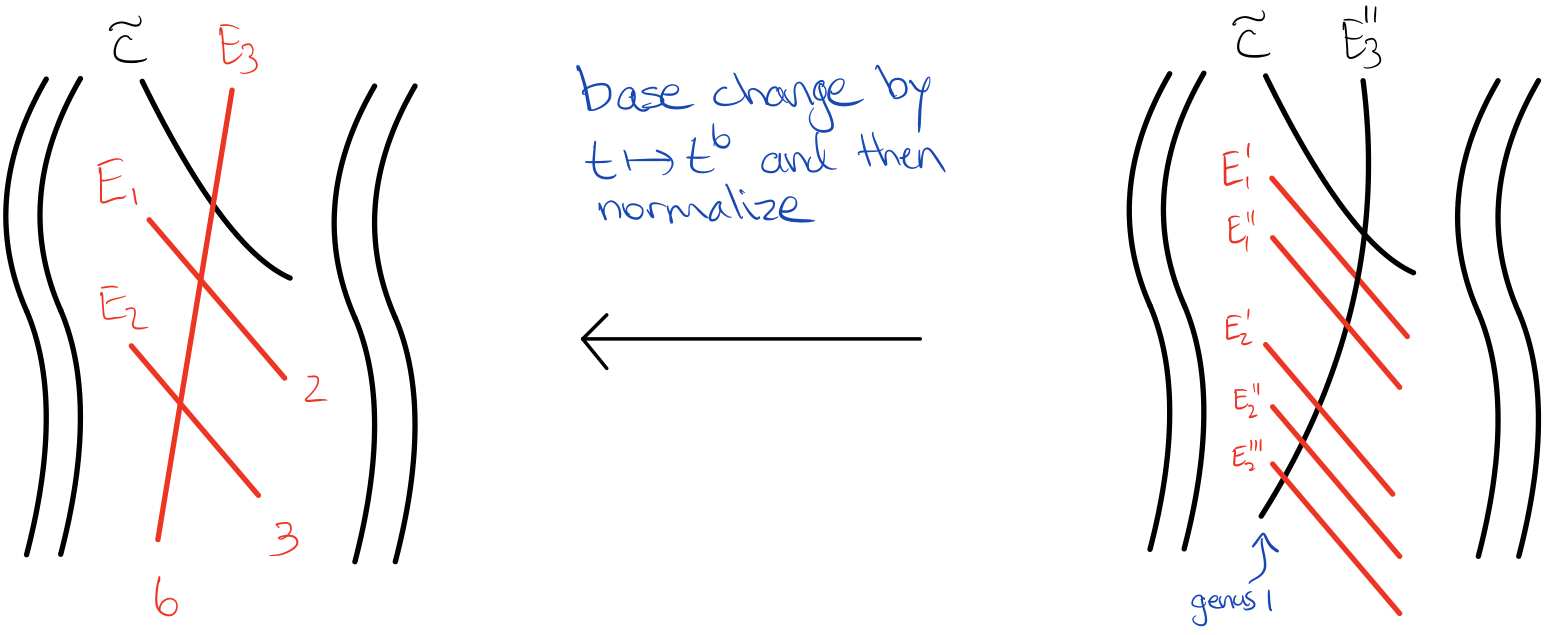
\includegraphics[width=.86\textwidth]{figures/reduction-step4.png}};
\begin{scope}[x={(im.south east)},y={(im.north west)}]
\fill[white] (0.36,0.63) rectangle (0.62,0.91);
\fill[white] (0.75,0.015) rectangle (0.83,0.1);
\node[fill=white,inner sep=1pt,font=\scriptsize,text=blue] at (0.5,0.83) {沿 $t\mapsto t^6$};
\node[fill=white,inner sep=1pt,font=\scriptsize,text=blue] at (0.5,0.71) {基变换并正规化};
\node[fill=white,inner sep=1pt,font=\scriptsize,text=blue] at (0.8,0.035) {亏格 $1$};
\end{scope}\end{tikzpicture}

\caption{(步骤 $4$) 接续图~\bookref{6.5.5}, 沿 $t\mapsto t^6$ 给出的 $\Delta'=\Spec\Bbbk[t]_{(t)}\to\Spec\Bbbk[t]_{(t)}=\Delta$ 对 $\mathcal C\to\Delta$ 作基变换, 再正规化. 中心纤维现已约化且仅有结点. $E_1$ 和 $E_2$ 的每个原像都是光滑有理曲线, $E_3$ 的原像 $E''_3$ 则是亏格 $1$ 曲线. 为理解此描述, 可将基变换分解为 $t\mapsto t^2$ 和 $t\mapsto t^3$ 的正规化基变换的复合; 见例~\bookref{6.5.13}.}\label{src:6.5.6}
\end{figure}
\textbf{步骤 $5$: 使标记点 $\sigma_i(0)\in\mathcal C_0$ 光滑且互异.}
反复爆破中心纤维 $\mathcal C_0$ 中标记点 $\sigma_i(0)$ 为奇点或相互碰撞的闭点, 则截面的严格变换成为中心纤维的互异光滑点. 将 $\mathcal C$ 换为爆破, 截面 $\sigma_i$ 换为严格变换后, 得到总族正则的预稳定族 $(\mathcal C\to\Delta,\allowbreak \sigma_i)$.
\begin{figure}[H]\centering\begin{tikzpicture}
\node[inner sep=0,anchor=south west] (im) at (0,0) {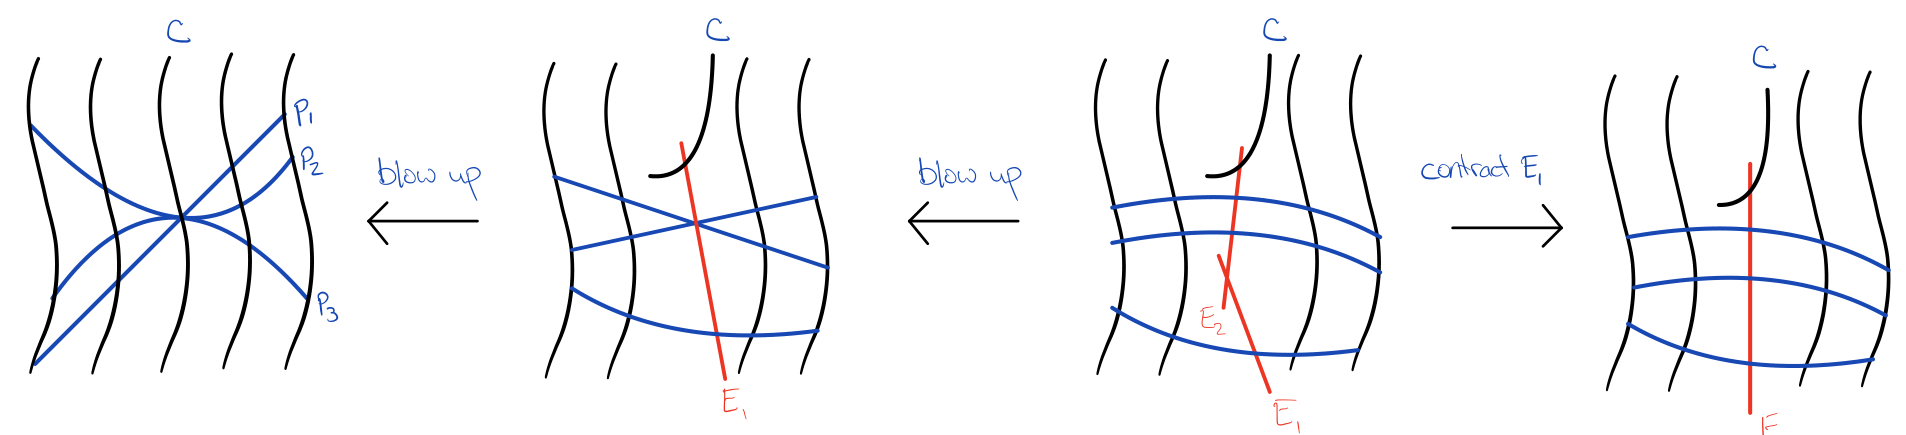
\includegraphics[width=.86\textwidth]{figures/reduction-step5.png}};
\begin{scope}[x={(im.south east)},y={(im.north west)}]
\fill[white] (0.18,0.52) rectangle (0.27,0.73);
\fill[white] (0.46,0.52) rectangle (0.55,0.73);
\fill[white] (0.74,0.52) rectangle (0.83,0.73);
\node[fill=white,inner sep=1pt,font=\scriptsize,text=blue] at (0.223,0.6) {爆破};
\node[fill=white,inner sep=1pt,font=\scriptsize,text=blue] at (0.506,0.6) {爆破};
\node[fill=white,inner sep=1pt,font=\scriptsize,text=blue] at (0.779,0.6) {收缩 $E_1$};
\end{scope}\end{tikzpicture}

\caption{(步骤 $5$) 考虑常值族 $C\times\Delta\to\Delta$, 截面局部为 $(\sigma_1,\allowbreak \sigma_2,\allowbreak \sigma_3)=(t^2,\allowbreak -t^2,\allowbreak 4t)$. 爆破两次后截面互不相交, 但中心纤维不稳定, 因为例外分支 $E_1\cong\mathbb P^1$ 仅有一个结点和一个标记点. 下一步将说明, 收缩有理桥 $E_1$ 即得稳定极限.}\label{src:6.5.7}
\end{figure}
\textbf{步骤 $6$: 收缩中心纤维中的有理尾和有理桥.}
预稳定族 $(\mathcal C\to\Delta,\allowbreak \sigma_i)$ 的中心纤维 $\mathcal C_0$ 稳定, 除非它含有有理尾或有理桥 (见定义~\bookref{6.3.12}). 若 $E\subseteq\mathcal C_0$ 是有理尾或带标记点的有理桥, 则 $E^2=-1$; 若 $E$ 是不带标记点的有理桥, 则 $E^2=-2$ (见注记~\bookref{6.3.16}). 由习题~\bookref{6.3.17}, 收缩每条有理尾和有理桥得到 $\Delta$ 上结点曲线族的态射 $\mathcal C\to\mathcal C'$. 令 $\sigma_i':\Delta\xrightarrow{\sigma_i}\mathcal C\to\mathcal C'$, 则 $n$-点曲线族 $(\mathcal C'\to\Delta,\allowbreak \sigma_i')$ 已经稳定! 也可用预稳定族的稳定收缩 (\bookref{6.6.6}) 构造此稳定族.
\end{proof}
\begin{figure}[H]\centering\begin{tikzpicture}
\node[inner sep=0,anchor=south west] (im) at (0,0) {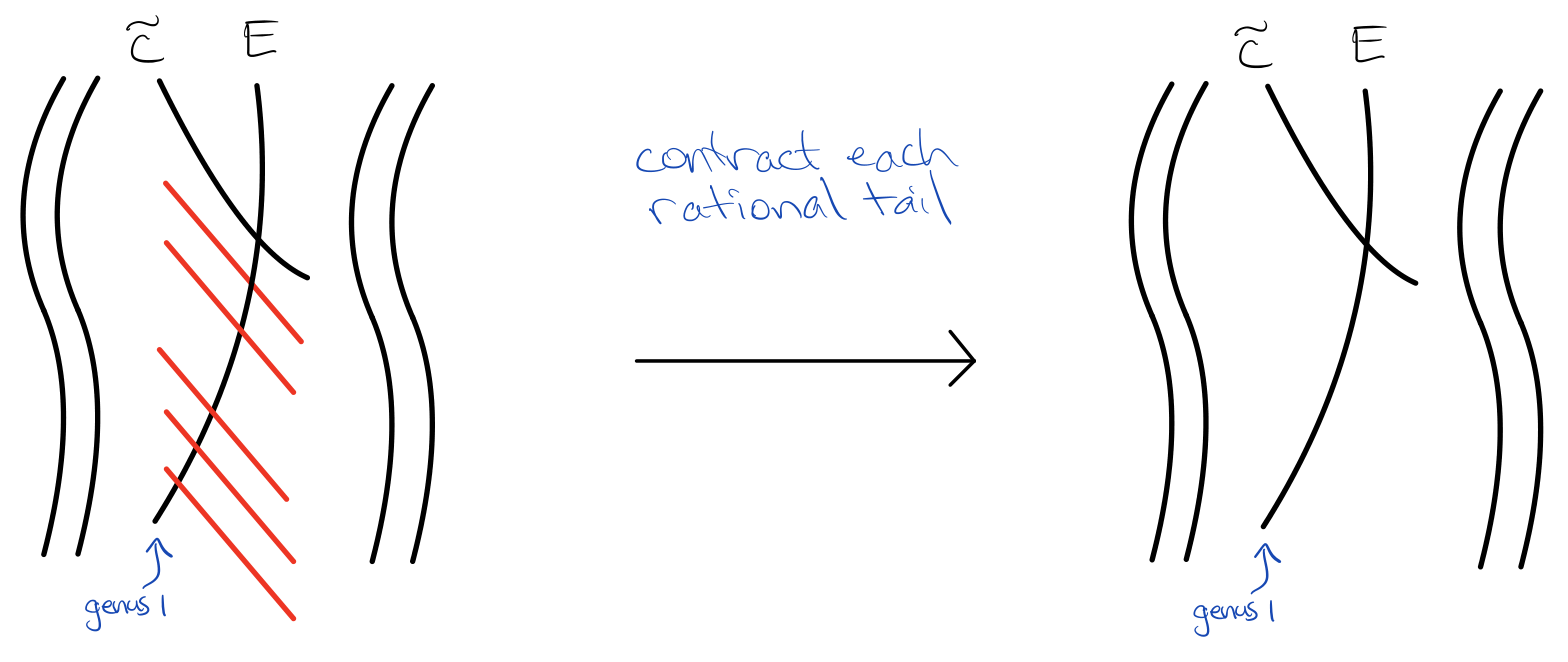
\includegraphics[width=.86\textwidth]{figures/reduction-step6.png}};
\begin{scope}[x={(im.south east)},y={(im.north west)}]
\fill[white] (0.37,0.62) rectangle (0.64,0.86);
\fill[white] (0.045,0.005) rectangle (0.13,0.085);
\fill[white] (0.75,0.005) rectangle (0.83,0.085);
\node[fill=white,inner sep=1pt,font=\scriptsize,text=blue] at (0.51,0.79) {收缩每条};
\node[fill=white,inner sep=1pt,font=\scriptsize,text=blue] at (0.51,0.7) {有理尾};
\node[fill=white,inner sep=1pt,font=\scriptsize,text=blue] at (0.085,0.055) {亏格 $1$};
\node[fill=white,inner sep=1pt,font=\scriptsize,text=blue] at (0.8,0.055) {亏格 $1$};
\end{scope}\end{tikzpicture}

\caption{(步骤 $6$) 接续图~\bookref{6.5.6}, 收缩每条红色有理尾得到稳定族. 中心纤维是原中心纤维 (带尖点) 的正规化 $\widetilde C$ 与椭圆曲线 $E$ 的结点并.}\label{src:6.5.8}
\end{figure}
若进行上述六步, 但在步骤 $6$ 中只收缩有理尾而保留有理桥, 则 Castelnuovo 收缩定理 (\bookref{B.2.6}) 保证总族仍正则. 这一重要变体称为\newterm{半稳定约化}{semistable reduction}.
\begin{theorem}[半稳定约化]\label{src:6.5.9}
设 $R$ 是离散赋值环, $K=\operatorname{Frac}(R)$, 并置 $\Delta=\Spec R$, $\Delta^*=\Spec K$. 若 $(\mathcal C^*\to\Delta^*,\allowbreak s_1^*,\allowbreak \ldots,\allowbreak s_n^*)$ 是 $n$-点\emph{光滑}曲线族, 则存在离散赋值环扩张 $R\to\allowbreak R'$ 及总族 $\mathcal C$ \emph{正则}的 $n$-点半稳定曲线族 $(\mathcal C\to\Delta'=\Spec R',\allowbreak s_1,\allowbreak \ldots,\allowbreak s_n)$, 延拓 $(\mathcal C^*\to\Delta^*,\allowbreak s_1^*,\allowbreak \ldots,\allowbreak s_n^*)$ 到 $K'=\operatorname{Frac}R'$ 的基变换.
\end{theorem}
\begin{remark}[特征 $p$ 下的证明]\label{src:6.5.10}
若 $R$ 的剩余域具有特征 $p>0$, 且中心纤维某些分支的重数被 $p$ 整除, 则上述稳定约化证明在步骤 $4$ 失效. 正特征下需要另一方法. 消解 $\mathcal C$ 的奇点并使 $(\mathcal C_0)_{\mathrm{red}}$ 仅有结点后 (如步骤 $3$), Artin 和 Winters 使 $\operatorname{Pic}(\mathcal C_{K'}^*)$ 的 $l$-挠子群对于充分大的素数 $l\ne p$ 同构于 $(\mathbb Z/l\mathbb Z)^{2g}$, 并证明这竟然迫使中心纤维约化且仅有结点! 见~\cite{AW71}, \cite[\S10.4]{Liu02} 和~\cite[Tag 0C2P]{SP}.
\end{remark}
\begin{example}[基变换必不可少]\label{src:6.5.11}
图~\bookref{6.5.5}, \bookref{6.5.6}, \bookref{6.5.8} 中尖点的稳定约化说明必须允许扩张离散赋值环. 事实上, 步骤 $3$ 后有一般光滑的族 $\mathcal C\to\Delta$, 总族 $\mathcal C$ 正则, 中心纤维 $\mathcal C_0$ 非约化. 假设存在稳定族 $\mathcal C'\to\Delta$, 使 $\mathcal C'|_{\Delta^*}\cong\mathcal C|_{\Delta^*}$. 消解 $\mathcal C'$ 的 $A_n$-奇点后, 有半稳定族 $\mathcal C''\to\Delta$, 其中 $\mathcal C''$ 正则, $\mathcal C''_0$ 半稳定 (特别地约化). 因为 $\mathcal C$ 与 $\mathcal C''$ 双有理, 取有理映射 $\mathcal C\dashrightarrow\mathcal C'$ 的图的闭包的奇点消解, 得到正则二维概形 $\mathcal D$ 和 $\Delta$ 上的双有理态射 $\mathcal D\to\mathcal C$, $\mathcal D\to\mathcal C''$. 由双有理映射的分解 (\bookref{B.2.4}), 每个态射分解为爆破的复合. 但 $\mathcal C$ 的任何爆破的中心纤维都非约化, $\mathcal C''$ 的任何爆破的中心纤维都约化, 这导致矛盾.
\end{example}
\subsection{显式稳定约化}\label{src:6.5.2-subsection}
在曲线几何的应用中, 常需明确描述稳定极限. 稳定约化的证明提供了策略, 但要得出显式描述还需仔细处理. 主要困难是确定步骤 $4$ 中全分歧扩张 $\Delta'\to\Delta$ 所给基变换 $\mathcal C'=\mathcal C\times_\Delta\Delta'$ 的正规化 $\widetilde{\mathcal C}'$. 常将 $\Delta'\to\Delta$ 分解为素数次基变换的复合更简单, 因为素数次正规化基变换 $\widetilde{\mathcal C}'\to\mathcal C$ 的分歧轨迹容易确定.
\begin{proposition}\label{src:6.5.12}
设 $p$ 是素数, $\mathcal C\to\Delta=\Spec R$ 是一般光滑的曲线族, 其中 $R$ 是含有 $p$ 次单位根的特征 $0$ 离散赋值环. 假设约化中心纤维 $(\mathcal C_0)_{\mathrm{red}}$ 仅有结点. 作为 $\mathcal C$ 上的除子, 写 $\mathcal C_0=\sum m_iD_i$, 其中 $m_i$ 是不可约分支 $D_i$ 的重数. 令 $\Delta'=\Spec R'\to\Spec R=\Delta$ 为 $p$ 次全非分歧扩张, 并置 $\mathcal C'=\mathcal C\times_\Delta\Delta'$, 正规化为 $\widetilde{\mathcal C}'$. 则 $\widetilde{\mathcal C}'\to\mathcal C$ 沿 $D_i$ 分歧当且仅当 $m_i$ 与 $p$ 互素. 若 $q'\in\widetilde{\mathcal C}'_0$ 是 $q\in D_i$ 的原像, 且 $q$ 是 $(\mathcal C_0)_{\mathrm{red}}$ 的光滑点, 则 $\widetilde{\mathcal C}'_0$ 在 $q'$ 附近的重数在 $p\mid m_i$ 时为 $m_i/p$, 否则为 $m_i$.
\end{proposition}
\begin{proof}
点 $q\in\mathcal C$ 有平展邻域和局部坐标 $x,\allowbreak y$, 使 $\mathcal C\to\Delta$ 描述为 $(x,\allowbreak y)\mapsto x^{m_i}$. 基变换 $\mathcal C'$ 在 $q'$ 附近平展局部描述为 $\Spec\Bbbk[x,\allowbreak y,\allowbreak t]/(x^{m_i}-t^p)$. 若 $p\mid m_i$, 则
\[
x^{m_i}-t^p=\prod_{i=0}^{p-1}(x^{m_i/p}-\rho^it),
\qquad\rho\text{ 为 }p\text{ 次单位根},
\]
其正规化有 $p$ 个光滑分支. 中心纤维 $\widetilde{\mathcal C}'_0$ 在 $q$ 的每个原像附近的重数为 $m_i/p$. 若 $m_i=pm'_i+r$, $0<r<p$, 则 $\Bbbk[x,\allowbreak y,\allowbreak t]/(x^{m_i}-t^p)$ 是整环, 正规化为
\[
\Bbbk[x,y,t']/(x^r-t'^p),\qquad t'=t/x^{m'_i}.
\]
所以 $\widetilde{\mathcal C}'\to\mathcal C$ 在 $q$ 处分歧. 中心纤维 $\widetilde{\mathcal C}'\to\Delta$ 由 $t=t'x^{m'_i}$ 定义, 在 $q$ 的唯一原像处的重数可计算为 $\dim_{\Bbbk}\Bbbk[x,\allowbreak t']/(x^r-t'^p,\allowbreak t'x^{m'_i})$. 因为 $t'^ix^j$ ($i=0,\allowbreak \ldots,\allowbreak p-1$, $j=0,\allowbreak \ldots,\allowbreak m'_i-1$) 与 $x^{m'_i},\allowbreak \ldots,\allowbreak x^{m'_i+r-1}$ 的并组成一组基, 重数为 $m_i$.
\end{proof}
\begin{example}[尖点的稳定约化]\label{src:6.5.13}
设 $\mathcal C\to\Delta=\Spec\Bbbk[t]_{(t)}$ 是一般光滑的族, 中心纤维 $C:=\mathcal C_0$ 退化出尖点 $y^2=x^3$, 且 $\mathcal C$ 在该奇点附近的局部方程为 $y^2=x^3+t$. 如图~\bookref{6.5.5} 所述, 对 $\mathcal C$ 作三次爆破, 得到族 $\mathcal C'\to\Delta$, 使 $(\mathcal C'_0)_{\mathrm{red}}$ 是正规化 $\widetilde C$ 与三个例外分支 $E_1,\allowbreak E_2,\allowbreak E_3$ 的结点并, 重数分别为 $1,\allowbreak 2,\allowbreak 3,\allowbreak 6$.
\end{example}
\begin{figure}[H]\centering\begin{tikzpicture}
\node[inner sep=0,anchor=south west] (im) at (0,0) {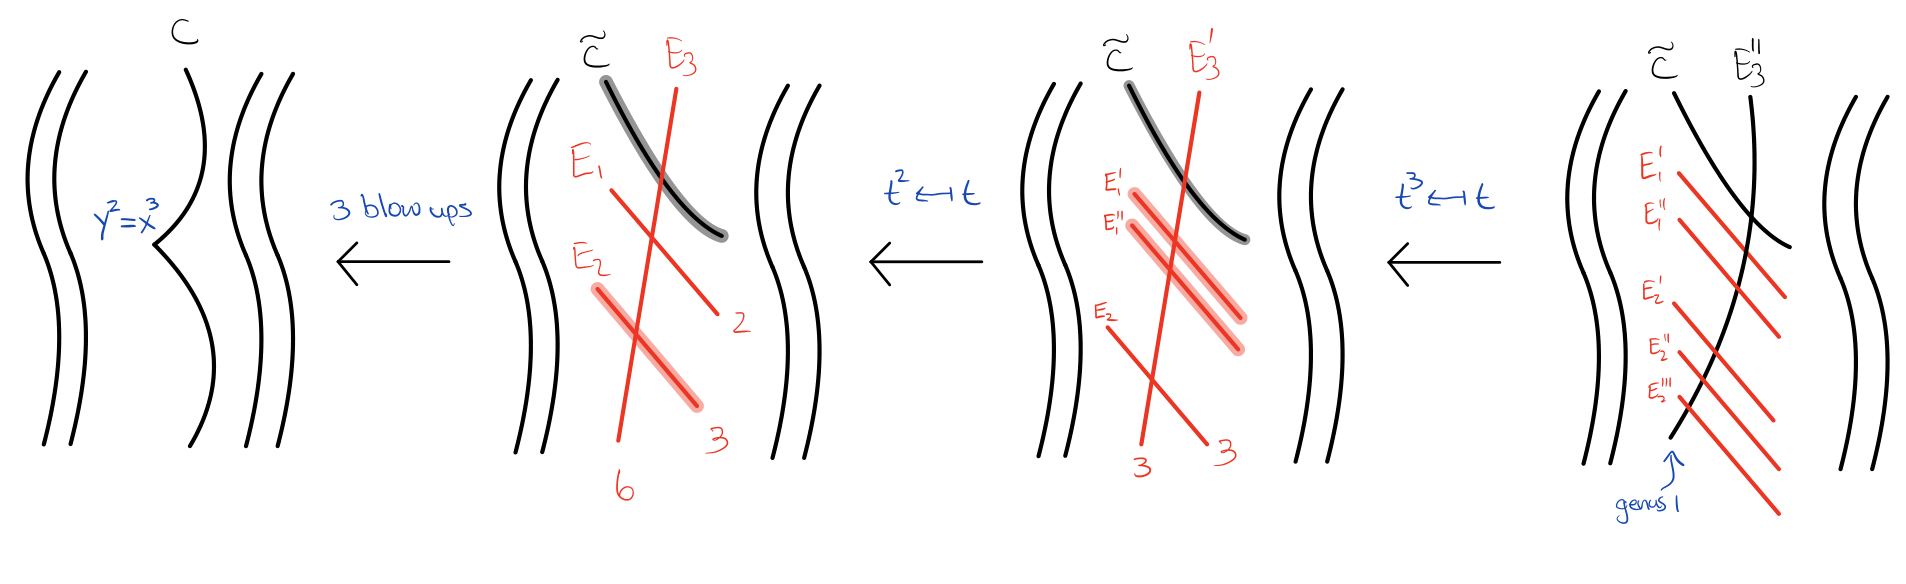
\includegraphics[width=.86\textwidth]{figures/reduction-cusp.png}};
\begin{scope}[x={(im.south east)},y={(im.north west)}]
\fill[white] (0.165,0.61) rectangle (0.26,0.75);
\fill[white] (0.46,0.62) rectangle (0.56,0.77);
\fill[white] (0.73,0.62) rectangle (0.81,0.77);
\fill[white] (0.845,0.09) rectangle (0.915,0.17);
\node[fill=white,inner sep=1pt,font=\scriptsize,text=blue] at (0.216,0.65) {$3$ 次爆破};
\node[fill=white,inner sep=1pt,font=\scriptsize,text=blue] at (0.5,0.675) {$t\mapsto t^2$};
\node[fill=white,inner sep=1pt,font=\scriptsize,text=blue] at (0.77,0.675) {$t\mapsto t^3$};
\node[fill=white,inner sep=1pt,font=\scriptsize,text=blue] at (0.88,0.13) {亏格 $1$};
\end{scope}\end{tikzpicture}

\caption{数字表示分支重数; 未标数字时重数为 $1$. 加粗分支表示正规化基变换的分歧轨迹.}\label{src:6.5.14}
\end{figure}
由命题~\bookref{6.5.12}, 第一次正规化基变换 $t\mapsto t^2$ 的分歧轨迹是 $\widetilde C$ 与 $E_2$ 的并. $E_1$ 的原像是两条光滑有理曲线的不交并 $E'_1\amalg E''_1$. $E_3$ 的原像 $E'_3$ 是在两点处分歧的 $E_3=\mathbb P^1$ 的二重覆盖, 所以 $E'_3=\mathbb P^1$, 但此时重数为 $2$. 第二次正规化基变换的分歧轨迹为 $\widetilde C\amalg E'_1\amalg E''_1$ (再次由命题~\bookref{6.5.12}). $E_2$ 的原像是三条光滑有理曲线的并, $E'_3$ 的原像 $E''_3$ 是 $E'_3=\mathbb P^1$ 的光滑三重覆盖, 在三点处分歧, 每点的分歧指数均为二. 由 Riemann--Hurwitz (\bookref{6.7.4}), $E''_3$ 的亏格 $g_{E''_3}$ 为 $1$:
\[
2g_{E''_3}-2=3(2(0)-2)+3(2)=0.
\]
最后如图~\bookref{6.5.8} 收缩五条有理尾, 稳定极限是光滑亏格 $g-1$ 曲线 $\widetilde C$ (原中心纤维的正规化) 与亏格 $1$ 曲线的结点并 $\widetilde C\cup E''_3$.
\begin{remark}\label{src:6.5.15}
稳定极限中究竟出现哪条椭圆曲线 $E''_3$, 稳定极限如何依赖退化的选择? 尖点的形变空间为 $y^2=x^3+a_1(t)x+a_0(t)$; 换言之, 问题是稳定极限如何依赖 $a_i(t)$. 例如, 若曲面的总族有奇点 (如 $y^2=x^{2k+1}+t^2$), 会发生什么? \cite[\S3.C]{HM98} 详细讨论了这些问题.
\end{remark}
\newpage
\begin{exercise}[很好的练习]\label{src:6.5.16}
\begin{enumerate}[(a)]
\item 求一般光滑的族退化出密切结点 $y^2=x^4$ 时的稳定极限.
\item 更一般地, 证明一般光滑的族退化出 $A_{2k}$-奇点 $y^2=x^{2k+1}$ (分别地, $y^2=x^{2k+2}$) 时, 稳定极限是亏格 $g-k$ 曲线与亏格 $k$ 超椭圆曲线的结点并, 在一个 Weierstrass 点 (分别地, 两个 Weierstrass 共轭点) 处粘接. 超椭圆曲线 $H$ 的 Weierstrass 点是二重覆盖 $H\to\mathbb P^1$ 的分歧点; 两点为 Weierstrass 共轭点是指它们的并是 $H\to\mathbb P^1$ 的一个纤维.
\end{enumerate}
\end{exercise}
\begin{example}[二重二次曲线的稳定约化]\label{src:6.5.17}
考虑一般光滑的族 $\mathcal C\to\Delta=\Spec\Bbbk[t]_{(t)}$, 其中 $\mathcal C\subseteq\mathbb P^2\times\Delta$ 由 $F^2+tG$ 定义, $F$ 是光滑二次曲线, $G$ 是光滑四次曲线. 中心纤维是 $F^2$ 定义的二重二次曲线. 总空间在 $F\cap G$ 的 $8$ 个交点 $p_1,\allowbreak \ldots,\allowbreak p_8$ 处各有一个局部方程为 $x^2+yt$ 的 $A_1$-奇点. 每个 $\sigma_i$ 经一次爆破消解, 例外除子 $E_i=\mathbb P^1$ 的重数为 $1$. 得到族 $\mathcal C_2\to\Delta$, 中心纤维作为除子为 $2C+\sum_iE_i$. 随后取分歧覆盖 $\Delta'\to\Delta$, $t\mapsto t^2$ 所给基变换 $\mathcal C_2\times_\Delta\Delta'$ 的正规化 $\mathcal C_3$. 由命题~\bookref{6.5.12}, $\mathcal C_3\to\mathcal C_2$ 沿 $E_i$ 的不交并分歧. $C$ 的原像是 $\mathbb P^1$ 的二重覆盖, 在 $8$ 个点 $\sigma_i$ 处分歧, 因而是光滑亏格 $3$ 超椭圆曲线.
\end{example}
\begin{figure}[H]\centering\begin{tikzpicture}
\node[inner sep=0,anchor=south west] (im) at (0,0) {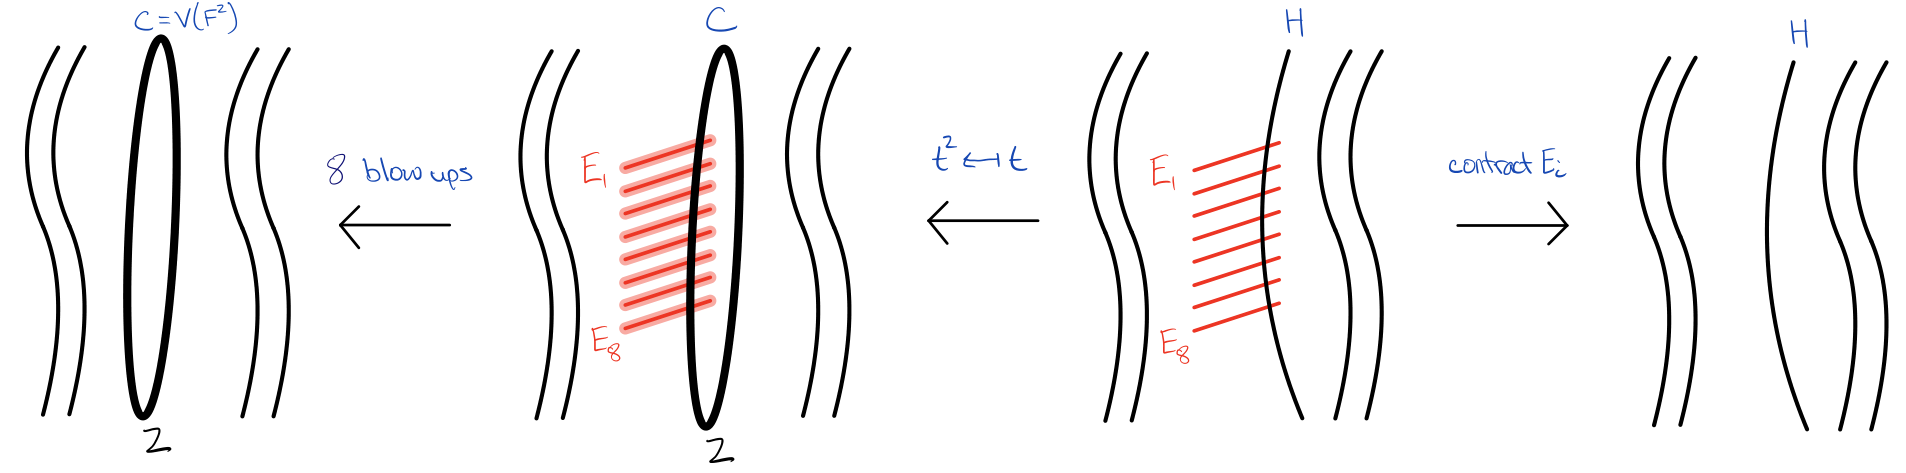
\includegraphics[width=.86\textwidth]{figures/reduction-double-conic.png}};
\begin{scope}[x={(im.south east)},y={(im.north west)}]
\fill[white] (0.16,0.58) rectangle (0.28,0.72);
\fill[white] (0.48,0.57) rectangle (0.56,0.72);
\fill[white] (0.74,0.57) rectangle (0.84,0.74);
\node[fill=white,inner sep=1pt,font=\scriptsize,text=blue] at (0.228,0.62) {$8$ 次爆破};
\node[fill=white,inner sep=1pt,font=\scriptsize,text=blue] at (0.5,0.62) {$t\mapsto t^2$};
\node[fill=white,inner sep=1pt,font=\scriptsize,text=blue] at (0.772,0.62) {收缩 $E_i$};
\end{scope}\end{tikzpicture}

\caption{退化为二重二次曲线 $C=V(F^2)$ 的一般光滑族 $F^2+tG$ 的稳定约化.}\label{src:6.5.18}
\end{figure}
\begin{exercise}[元习题]\label{src:6.5.19}
阅读~\cite[\S3.C]{HM98} 的论述并完成其中的习题.
\end{exercise}
\subsection{\texorpdfstring{$\overline{\mathcal M}_{g,\allowbreak n}$ 的固有性}{稳定曲线模叠 的固有性}}\label{src:6.5.3-subsection}
稳定约化 (\bookref{6.5.1}) 蕴涵 $\overline{\mathcal M}_{g,\allowbreak n}$ 的固有性赋值判据中的存在性部分. 还需证明稳定极限唯一, 即 $\overline{\mathcal M}_{g,\allowbreak n}$ 分离.
\begin{proposition}\label{src:6.5.20}
设 $R$ 是离散赋值环, $K=\operatorname{Frac}(R)$, 并置 $\Delta=\Spec R$, $\Delta^*=\Spec K$. 若 $(\mathcal C\to\Delta,\allowbreak \sigma_1,\allowbreak \ldots,\allowbreak \sigma_n)$ 和 $(\mathcal D\to\Delta,\allowbreak \tau_1,\allowbreak \ldots,\allowbreak \tau_n)$ 是 $n$-点稳定曲线族, 则 $\Delta^*$ 上每个与截面的限制相容 (即 $\tau_i^*=\alpha^*\circ\sigma_i^*$) 的同构 $\alpha^*:\mathcal C\times_\Delta\Delta^*\to\mathcal D\times_\Delta\Delta^*$, 均延拓为唯一的 $\Delta$ 上同构 $\alpha:\mathcal C\to\mathcal D$, 满足 $\tau_i=\alpha\circ\sigma_i$.
\end{proposition}
\begin{proof}
为简单起见, 处理无标记点 ($n=0$) 的情形. 先断言可归结到一般纤维 $\mathcal C^*\cong\mathcal D^*$ 在 $\Delta^*$ 上光滑, 其中 $\mathcal C^*=\mathcal C\times_\Delta\Delta^*$. 采用稳定约化 (\bookref{6.5.1}) 证明的步骤 $1$ 中归结到一般光滑情形的同一策略. 由平坦下降, 只需在离散赋值环扩张 $\Delta'\to\Delta$ 后构造 $\alpha:\mathcal C\to\mathcal D$; 事实上, 同构 $\alpha':\mathcal C\times_\Delta\Delta'\to\mathcal D\times_\Delta\Delta'$ 因 $\mathcal D\to\Delta$ 分离而满足余圈条件, 从而下降为同构 $\alpha$. 因而可假设 $\mathcal C^*\cong\mathcal D^*$ 的每个结点由 $K$-点给出, 在正规化下的原像为两个 $K$-点. 每个结点延拓为截面 $\Delta\to\mathcal C$, $\Delta\to\mathcal D$. 带标记的正规化 $\widetilde{\mathcal C}$, $\widetilde{\mathcal D}$ 各为带标记稳定族的不交并. 若 $\mathcal C^*\to\mathcal D^*$ 延拓为同构 $\widetilde\alpha:\widetilde{\mathcal C}\to\widetilde{\mathcal D}$, 则 $\alpha$ 下降为同构 $\mathcal C\to\mathcal D$. 或者利用 $\mathcal M_{g,\allowbreak n}\subseteq\overline{\mathcal M}_{g,\allowbreak n}$ 稠密 (稍后定理~\bookref{6.7.30} 证明), 只需在 $\Delta^*\to\overline{\mathcal M}_{g,\allowbreak n}$ 经过 $\mathcal M_{g,\allowbreak n}$ 分解的条件下检验分离性的赋值判据 (习题~\bookref{5.6.7}).

令 $\widetilde{\mathcal C}\to\mathcal C$ 和 $\widetilde{\mathcal D}\to\mathcal D$ 为极小消解 (定理~\bookref{B.2.2}). 令 $\Gamma$ 为 $(\mathrm{id},\allowbreak \alpha^*):\mathcal C^*\to\widetilde{\mathcal C}\times_\Delta\widetilde{\mathcal D}$ 的像的闭包, $\widetilde\Gamma\to\Gamma$ 为其极小消解. 得到交换图
\begin{equation}\label{src:6.5.21}
\begin{tikzcd}[column sep=small,row sep=small]
&\widetilde{\mathcal C}\arrow[r]&\mathcal C\arrow[dr]&\\
\widetilde\Gamma\arrow[ur]\arrow[dr]&&&\Delta\\
&\widetilde{\mathcal D}\arrow[r]&\mathcal D\arrow[ur]&
\end{tikzcd}
\end{equation}
给出两种论证说明存在延拓 $\alpha^*$ 的同构 $\alpha:\mathcal C\to\mathcal D$. 第一种: $\mathcal C$ (分别地 $\mathcal D$) 在中心纤维的结点附近的局部结构是形如 $xy=t^{n+1}$ 的 $A_n$-奇点, 其中 $t\in R$ 是一致化参数. 每个结点在 $\widetilde{\mathcal C}\to\mathcal C$ (分别地 $\widetilde{\mathcal D}\to\mathcal D$) 下的原像是有理桥链 $E_1\cup\cdots\cup E_n$, $E_i^2=-2$. 因为 $\mathcal C$, $\mathcal D$ 是稳定曲线族, 它们不含光滑有理 $-1$ 曲线, 所以 $\widetilde{\mathcal C}$, $\widetilde{\mathcal D}$ 也不含这样的曲线. 由双有理映射的分解 (定理~\bookref{B.2.4}), $\widetilde\Gamma\to\widetilde{\mathcal C}$ 和 $\widetilde\Gamma\to\widetilde{\mathcal D}$ 都是有限次闭点爆破的复合. 因为 $\widetilde\Gamma\to\Gamma$ 是极小消解, $\widetilde\Gamma$ 不含同时被两个态射收缩的光滑有理 $-1$ 曲线. 断言这两个态射都是同构. 这将完成证明, 因为 $\mathcal C$, $\mathcal D$ 均由收缩 $\widetilde{\mathcal C}\cong\widetilde{\mathcal D}$ 的光滑有理 $-2$ 曲线得到.

为证断言, 假设例如 $\widetilde\Gamma\to\widetilde{\mathcal C}$ 不是同构. 则存在不被 $\widetilde\Gamma\to\widetilde{\mathcal D}$ 收缩的光滑有理 $-1$ 曲线 $E\subseteq\widetilde\Gamma$. 令 $E_{\widetilde{\mathcal D}}\subseteq\widetilde{\mathcal D}$ 为它的像. 爆破只会减小自交数 (事实上, 若 $E_{\widetilde{\mathcal D}}$ 在 $\Gamma$ 中的原像写成 $E+F$, 则投影公式给出 $E_{\widetilde{\mathcal D}}^2=E\cdot(E+F)=E^2+E\cdot F$), 所以 $E_{\mathcal D}^2\geq E^2=-1$. 另一方面, 例外曲线的 Hodge 指数定理 (\bookref{B.2.5}) 给出 $E_{\mathcal D}^2\leq-1$. 因而 $E_{\mathcal D}^2=-1$. 但 $E_{\mathcal D}\subseteq\widetilde{\mathcal D}$ 不是光滑有理 $-1$ 曲线, 故必有奇点, 复合 $\widetilde\Gamma\to\widetilde{\mathcal D}$ 中某次爆破必在 $E_{\mathcal D}$ 的奇点处进行. 这意味着例外轨迹 $F$ 与 $E$ 非平凡相交, 从而 $E_{\mathcal D}^2\geq E^2+1$, 矛盾.

也可如下论证. 光滑射影曲面的双有理映射 $\widetilde\Gamma\to\widetilde{\mathcal C}$ 和 $\widetilde\Gamma\to\widetilde{\mathcal D}$ 在余维 $2$ 处是同构. 相对对偶化层是线丛, 因而对每个非负整数 $k$, 多重典范截面有认同
\[
\Gamma(\widetilde{\mathcal C},\omega_{\widetilde{\mathcal C}/\Delta}^{\otimes k})
\cong\Gamma(\widetilde\Gamma,\omega_{\widetilde\Gamma/\Delta}^{\otimes k})
\cong\Gamma(\widetilde{\mathcal D},\omega_{\widetilde{\mathcal D}/\Delta}^{\otimes k})
\]
(参见~\cite[定理 II.8.19]{Har77}). 由 $\mathcal C$, $\mathcal D$ 是 $\Delta$ 上族 $\widetilde{\mathcal C}$, $\widetilde{\mathcal D}$ 的稳定收缩 (定理~\bookref{6.6.6}), 即多重典范截面分次环的 $\operatorname{Proj}$, 得到延拓 $\alpha^*:\mathcal C^*\to\mathcal D^*$ 的同构
\[
\mathcal C\xrightarrow{\sim}\operatorname{Proj}\bigoplus_k\Gamma(\widetilde{\mathcal C},\omega_{\widetilde{\mathcal C}/\Delta}^{\otimes k})
\xrightarrow{\sim}\operatorname{Proj}\bigoplus_k\Gamma(\widetilde{\mathcal D},\omega_{\widetilde{\mathcal D}/\Delta}^{\otimes k})
\xrightarrow{\sim}\mathcal D.
\]
另见~\cite[引理 1.12]{DM69}, \cite[引理 10.5.1]{ACG11} 和~\cite[Tag 0E97]{SP}.
\end{proof}
\begin{exercise}[细节]\label{src:6.5.22}
将上述证明推广到有标记点的情形.
\end{exercise}
虽然我们只在特征 $0$ 下证明了稳定约化 (\bookref{6.5.1}), 仍在 $\mathbb Z$ 上陈述下一个结果.
\begin{theorem}[$\overline{\mathcal M}_{g,\allowbreak n}$ 和 $\overline M_{g,\allowbreak n}$ 的固有性]\label{src:6.5.23}
若 $2g-2+n>0$, 则 Deligne--Mumford 叠 $\overline{\mathcal M}_{g,\allowbreak n}$ 在 $\Spec\mathbb Z$ 上固有. 此外, 存在粗模空间 $\overline{\mathcal M}_{g,\allowbreak n}\to\overline M_{g,\allowbreak n}$, 其中 $\overline M_{g,\allowbreak n}$ 是 $\Spec\mathbb Z$ 上固有的代数空间.
\end{theorem}
\begin{proof}
因为 $\overline{\mathcal M}_{g,\allowbreak n}$ 拟分离 (习题~\bookref{6.4.18}), 可应用固有性的赋值判据 (\bookref{4.8.7}). 稳定约化 (\bookref{6.5.1}) 给出极限的存在性, 命题~\bookref{6.5.20} 给出唯一性. 因为 $\overline{\mathcal M}_{g,\allowbreak n}$ 分离, Keel--Mori 定理 (\bookref{5.4.6}) 给出粗模空间 $\overline{\mathcal M}_{g,\allowbreak n}\to\overline M_{g,\allowbreak n}$, 其中 $\overline M_{g,\allowbreak n}$ 是 $\Spec\mathbb Z$ 上分离有限型的代数空间. 由于 $\overline{\mathcal M}_{g,\allowbreak n}$ 在 $\Spec\mathbb Z$ 上固有, $\overline M_{g,\allowbreak n}$ 也固有.
\end{proof}
\begin{exercise}\label{src:6.5.24}
证明 $\overline{\mathcal M}_{g,\allowbreak n}\times_{\mathbb Z}\mathbb F_p$ 的粗模空间是 $\overline M_{g,\allowbreak n}\times_{\mathbb Z}\mathbb F_p$ 的正规化.
\end{exercise}
\newpage
\begin{question}[未解决]\label{src:6.5.25}
$\overline M_{g,\allowbreak n}\times_{\mathbb Z}\mathbb F_p$ 是否为 $\overline{\mathcal M}_{g,\allowbreak n}\times_{\mathbb Z}\mathbb F_p$ 的粗模空间?\footnote{见 \url{https://mathoverflow.net/questions/9981/coarse-moduli-spaces-over-z-and-f-p} 和 \url{https://mathoverflow.net/questions/72903/what-is-m-g-over-a-finite-field-really}.}
\end{question}
